% !TEX encoding = UTF-8
% !TEX TS-program = pdflatex
% !TEX root = ../tesi.tex

%**************************************************************
\chapter{Introduzione ai casi d'uso per l'analisi comparativa}
\label{cap:casi-uso}
%**************************************************************

\intro{Illustrazione del prototipo realizzato, prime considerazioni su di esso.
        Successivamente caso d'uso di SushiLab, migrazione e considerazioni.}\\
\subsection{Confronto con stakeholder}
Parlo confronto stakeholder....
\section{Prototipo}
\textcolor{red}{FORSE QUESTA PARTE VA SU UNO DEI PRIMI DUE CAPITOLI.... INTANTO LASCIO QUA.}\\\\
Prima di procedere con la spiegazione nella progettazione, realizzazione e migrazione del prototipo vanno fatte delle premesse.\\
Si tratta di un prototipo realizzato al fine di:
\begin{itemize}
  \item familiarizzare con le tecnologie Spring e Angular per la realizzazione rispettivamente di backend e frontend, il tutto in preparazione alla migrazione dell'applicativo aziendale riportato al punto \ref{sushi-lab};
  \item familiarizzare con la realizzazione delle API sia con lo stile architetturale REST, che con il linguaggio di query GraphQL;
  \item avere un caso d'uso ulteriore a conferma delle analisi che verranno poi ricavate dalla migrazione dell'applicativo SushiLab;
\end{itemize}
Per questi motivi si tratta di un prototipo specifico che mira alla realizzazione delle API e al loro massimo utilizzo.\\\\
Il prototipo che è stato scelto di realizzare è un applicazione client-server con funzione di gestionale. Deve permettere di gestire gli impiegati e i progetti ai quali stanno lavorando, il tutto in diverse sedi con diversi dipartimenti.
\subsection{Progettazione del prototipo}
\subsubsection*{Architettura generale dell'applicativo}
L'applicativo utilizza la classica architettura introdotta al punto \ref{client-server} con un backend sviluppato con Spring Boot e il frontend sviluppato con Angular. In figura \ref{prototype-architecture} è possibile visualizzare l'architettura del prototipo con API REST:
\begin{figure}[!h]
\centering
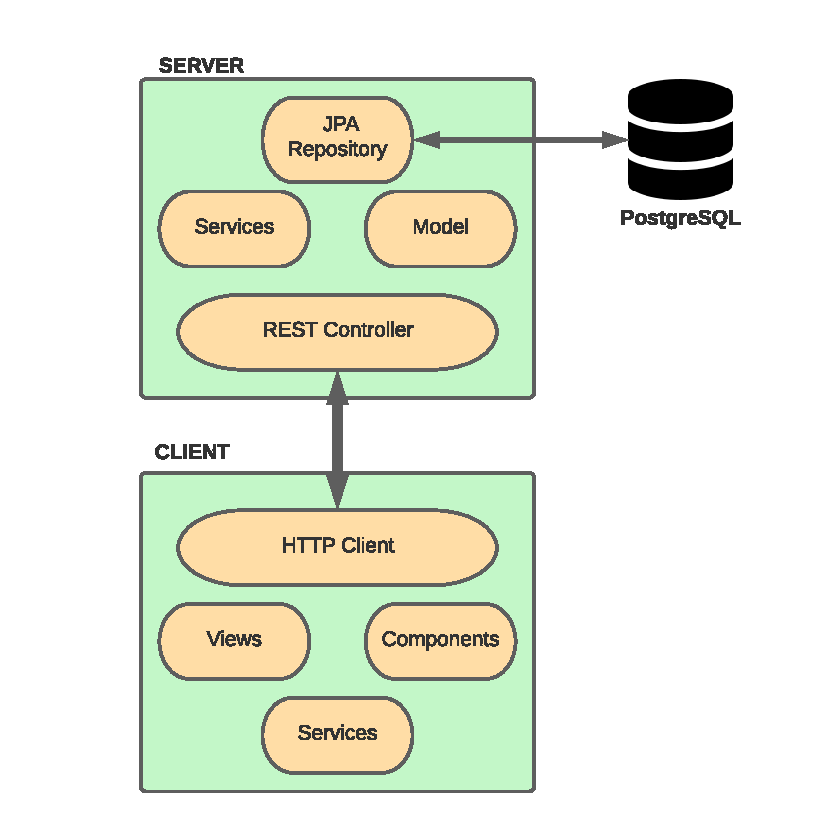
\includegraphics[width=0.6\linewidth]{immagini/prototype_architecture.pdf}
\caption{Architettura del prototipo di Web Application.}
\label{prototype-architecture}
\end{figure}
Verrà dunque realizzato un server con framework Spring Boot e la Web Application con framework Angular. Per maggiori informazioni riguardo alle tecnologie consultare il capitolo \ref{tecnologie}.
\subsubsection*{Architettura del server}
% Qui devo parlare di:
%   - pattern controller - service - repository;
%   - architettura del backend con hibernate, postgreSQL.
\paragraph{Controller - Service - Repository}
È stato deciso di seguire il pattern controller - service - repository per la realizzazione del server del prototipo. Questa scelta è stata presa in quanto è consigliato nello sviluppo del backend con framework Spring Boot. Inoltre il pattern rispetta perfettamente il principio di "Separation Of Concerns".\\
Il pattern prevedere la gestione delle entità e delle chiamate alle API attraverso tre strati:
\begin{itemize}
  \item \textbf{Controller layer}: si trova in cima all'immagine \ref{controller-service-repository}, è l'unico responsabile della interazione con entità esterne, inoltre gestisce le interfacce REST e invoca lo strato di servizio;
  \item \textbf{Service layer}: è lo strato tra controller e repository, si occupa della business logic e qualora sia necessario visualizzare, salvare, modificare o eliminare dati allora comunica con lo strato di persistenza;
  \item \textbf{Repository layer}: si tratta dello strato inferiore dell'architettura, si occupa della gestione dei dati e delle loro modifiche. Lo strato di repository inoltre si occupa della comunicazione e gestione del database.
\end{itemize}
%%%% IMG
\begin{figure}[!h]
\centering
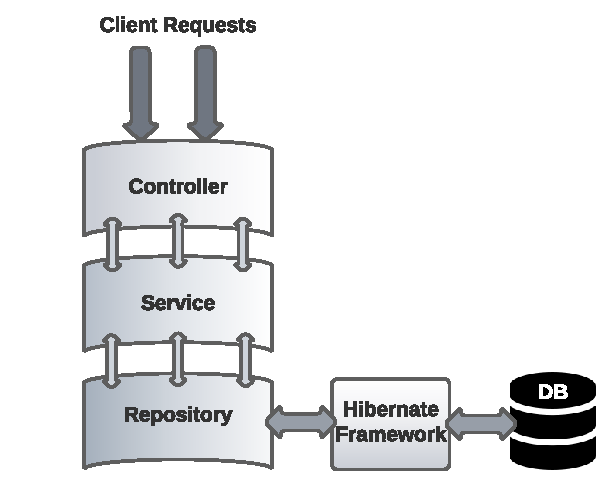
\includegraphics[width=0.8\linewidth]{immagini/controller_service_repository.pdf}
\caption{Architettura interna backend.}
\label{controller-service-repository}
\end{figure}
\textcolor{red}{PARLARE E INSERIRE QUI DIAGRAMMA DI SEQUENZA}
%%%% IMG
\paragraph{Entità e relazioni}
\label{entity-relation}
Trattandosi di un gestionale aziendale semplificato, sono previste solo quattro entità principali, queste sono:
\begin{itemize}
  \item \textbf{Employee}: l'impiegato che può lavorare ad uno o più progetti e in un dipartimento;
  \item \textbf{Project}: un progetto aziendale a cui partecipano più impiegati;
  \item \textbf{Site}: si tratta di una sede aziendale, può avere più dipartimenti;
  \item \textbf{Department}: un dipartimento che appartiene ad una sede.
\end{itemize}
%%% IMG
\FloatBarrier
\begin{figure}[!ht]
\centering
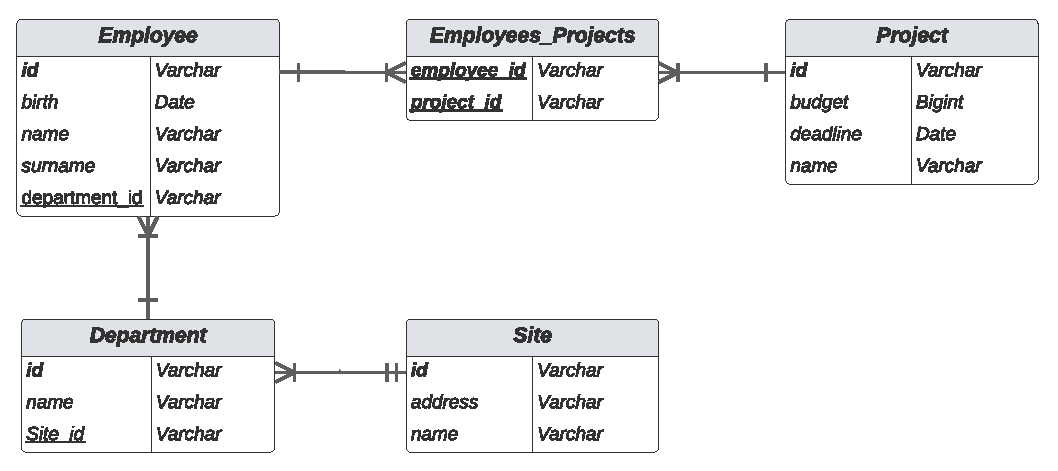
\includegraphics[width=0.8\linewidth]{immagini/ER_prototype.pdf}
\caption{Diagramma ER del prototipo.}
\label{ER-prototype}
\end{figure}
\FloatBarrier
%%% IMG
Ciascuna entità è caratterizzata da i campi presenti in figura \ref{ER-prototype} dove è stato utilizzato il linguaggio UML. Le relazioni presenti tra le varie entità sono:
\begin{itemize}
  \item \textbf{many to many}: è presente tra Employee e Project, infatti ciascun impiegato può lavorare a più progetti e ciascun progetto può avere più impiegati al quale ci lavorano;
  \item \textbf{one to many}: è presente tra due coppie di entità:
    \begin{itemize}
      \item tra Employee e Department, infatti ciascun impiegato può lavorare in uno o nessun dipartimento, mentre ciascun dipartimento può ospitare più impiegati;
      \item tra Department e Site, ciascun dipartimento può appartenere esclusivamente ad una sede, mentre ciascuna sede può esser composta da più dipartimenti.
    \end{itemize}
\end{itemize}
\subsubsection*{Realizzazione e testing server}
Durante la realizzazione viene seguito il percorso inverso rispetto a quanto visto nell'immagine \ref{controller-service-repository}, infatti la realizzazione avviene partendo dallo strato di persistenza, dunque dalla creazione delle entità e delle repositoryes.
\paragraph{Entità e repository}
A ciascun entità nel database viene fatta corrispondere una classe in Java. Per questo devono essere realizzate 4 classi rappresentanti le entità Employee, Project, Department e Site.\\
Ciascuna classe entità implementa la classe \textit{Serializable}, così facendo è possibile serializzare i dati in flussi di byte. La serializzazione viene utilizzata poiché si tratta di dati che dovranno essere memorizzati nel database, dunque è necessario serializzarli poiché abbandonano la Java Virtual Machine. Viene inoltre utilizzato un \textit{serialVersionUID} per attribuire una versione a ciascuna classe di entità serializzabile, necessario per riconoscere quando nella comunicazione con il database o con altri moduli esterni la versione dell'entità risulta differente, si tratta dunque di entità che non corrispondono totalmente, in quel caso viene ritornato un erorre \textit{InvalidClassException}.\\
Le quattro entità descritte quindi nel capitolo \ref{entity-relation} dovranno essere implementate come classi, segue l'esempio dell'implementazione della classe Employee:
%%% IMG
\FloatBarrier
\begin{figure}[!ht]
\centering
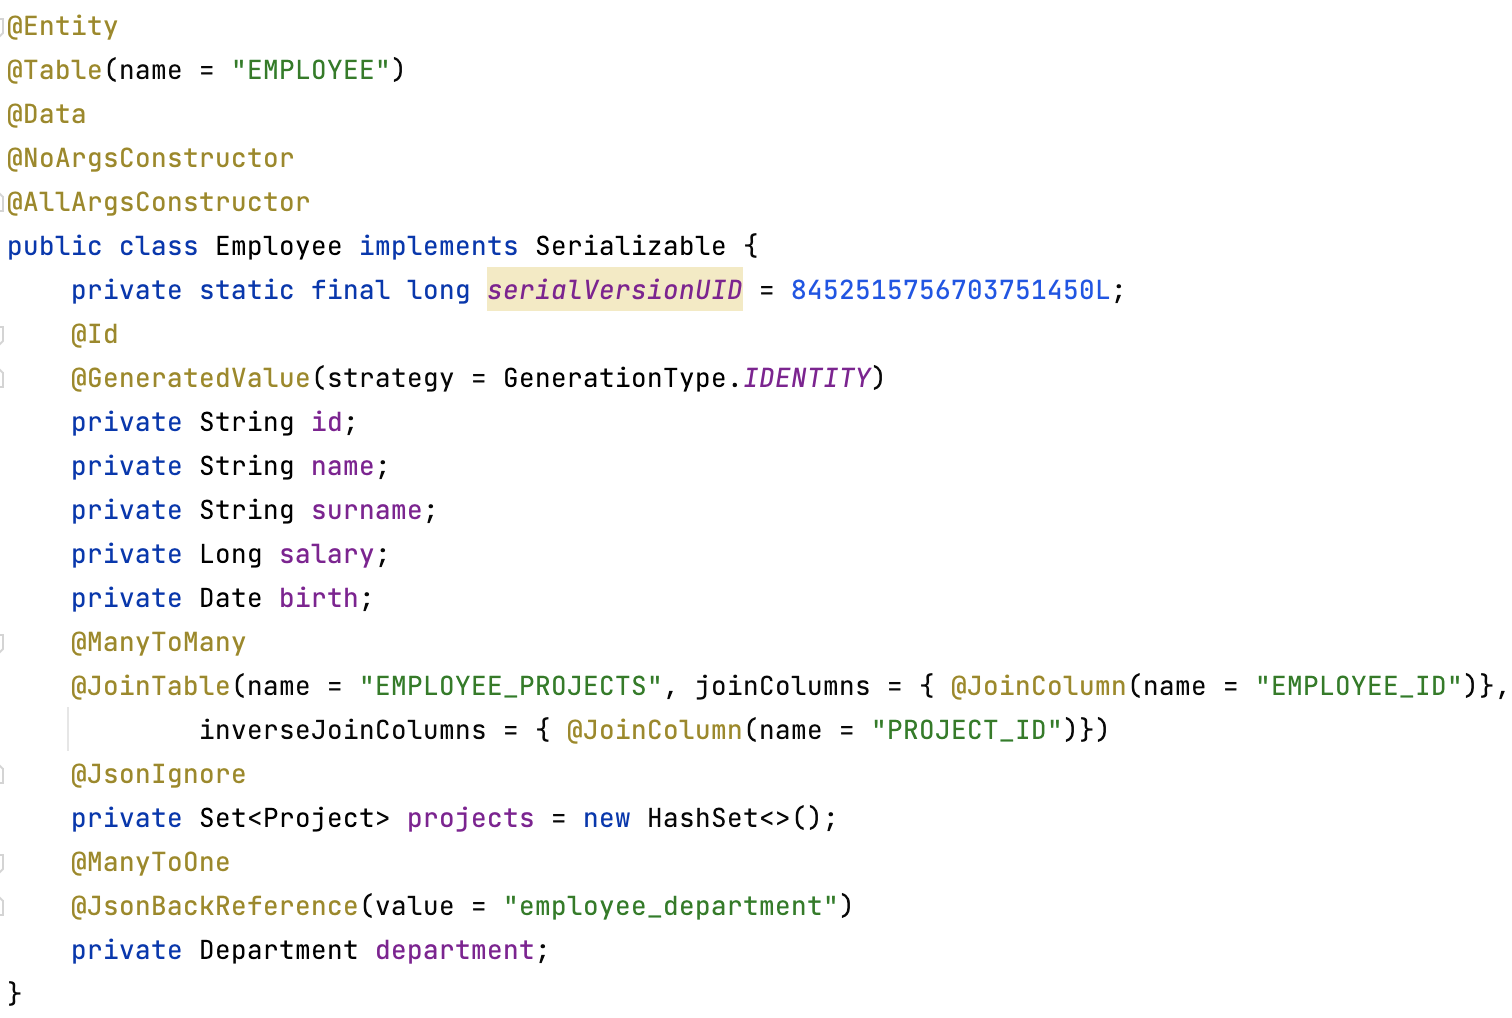
\includegraphics[width=0.9\linewidth]{immagini/employee_entity.png}
\caption{Esempio di implementazione dell'entità Employee in Spring Boot.}
\label{employee-entity-definition}
\end{figure}
\FloatBarrier
%%% IMG
Vengono attribuite alla classe Employee diverse annotazioni Spring, tra queste:
\begin{itemize}
  \item \textbf{@Entity}: si tratta dell'annotazione che permette di mappare la classe Employee come una corrispondente tabella nel database. Questa annotazione è resa disponibile dal modulo Spring Data JPA il quale implementa la specifica delle Java Persistence API attraverso Hibernate ORM e permette dunque il mapping della classi con corrispettive entità nel database;
  \item \textbf{@Table}: questa annotazione permette di specificare il  nome della tabella generata o presente nel database durante la sua creazione o aggiornamento;
  \item \textbf{@Data}: grazie alla libreria \textit{lombok} è possibile, attribuendo alla classe questa annotazione, generare automaticamente tutti i metodi get e set per tutti i campi della classe;
  \item \textbf{@NoArgConstructor e @AllArgConstructor}: permettono di generare tutti le combinazioni di costruttori con parametri e quello senza parametri.
\end{itemize}
Spostando invece il focus sui campi della classe Employee in figura \ref{employee-entity-definition}, possiamo notare che il campo \textit{id} ha due annotazioni associate. La annotazione \textbf{@Id} permette di specificare nel mapping che si tratta della chiave primaria, mentre l'annotazione \textbf{@GeneratedValue} permette di specificare che quando una nuova istanza di una entità viene creata, deve essere generato un nuovo id randomico.\\\\
Proseguendo sono presenti tutte le dichiarazioni dei vari campi dati dell'entità Employee e infine, troviamo le relazioni che Employee ha con le enetità Project e Department. Anche in questo caso le annotazioni fornite dalla specifica JPA permettono di specificare nel dettaglio le varie relazioni. Sono dunque presenti le annotazioni:
\begin{itemize}
  \item \textbf{@ManyToMany} e \textbf{@ManyToOne}: queste specificano il tipo di relazione che è presente con le altre entità, sono rispettivamente associate ai campi \textit{projects}, con il quale Employee ha una relazione molti a molti e infine al campo \textit{department}, con il quale Employee ha una relazione molti a uno;
  \item \textbf{@JoinTable}: è associata al campo \textit{projects}, e poiché le relazioni molti a molti necessitano di una ulteriore tabella per la memorizzazione di tutte le associazioni, questa annotazione permette di specificarne il nome, ovvero \textit{EMPLOYEE-PROJECTS} e i nomi delle due colonne, ovvero \textit{EMPLOYEE-ID} e \textit{PROJECT-ID};
  \item \textbf{@JsonIgnore}: associato al campo \textit{projects}, permette di escluderlo dalla serlizzazione;
  \item \textbf{@JsonBackReference}: associato al campo \textit{department}, permette di dare una direzionalità alla relazione molti a uno con Department, fondamentale per evitare il problema della ricorsione infinita \textcolor{red}{(QUI NON SO SE SPIEGARE)}.
\end{itemize}
Analogamente sono state realizzate le classi corrispondenti alle entità Project, Department e Site.\\\\
A questo punto si procede con la realizzazione delle classi repository: ciascuna entità ha una propria repository corrispondente. Dunque viene estesa l'interfaccia \textbf{JPArepository<T, ID>} con T il tipo della entità che si vuole gestire, mentre ID è il tipo della chiave primaria dell'entità T. La repository JPA deriva da diverse interfacce, tra le quali:
\begin{itemize}
  \item \textbf{CrudRepository<T, ID>}: la quale contiene le API per gestire le classiche operazioni CRUD;
  \item \textbf{PagingAndSortingRepository<T, ID>}: la quale contiene le API per gestire la pagination e il sorting;
\end{itemize}
Dunque estendendo la JPARepository per ciascun tipo è possibile avere a disposizione diversi metodi per eseguire operazioni già implementate come: findAll, count, existById, SaveAndFlush, ecc...\\
Qualora invece si volesse rendere disponibili nuovi metodi è possibile dichiararli nell'estensione della repository, senza necessariamente implementarli, poiché è sufficiente attribuire il nome corretto al metodo. Più specificatamente il nome del metodo corrispondente alla query che si vuole render disponibile è composto da un introducer che può essere uno tra: \textit{find}, \textit{read}, \textit{query}, \textit{count} o \textit{get}, e successivamente il criterio seguito dalla keywork \textit{By}, quindi ad esempio se si volesse fare una ricerca per salario, è sufficiente dichiarare un metodo chiamato \textit{findBySalary}. \\
Infine ritroviamo il caso in qui si vuole realizzare una query complessa o personalizzata, in questo caso ci viene in aiuto la annotazione \textbf{@Query} alla quale è possibile passare come attributo la query che desideriamo in linguaggio JPQL. Di seguito è possibile visualizzare quanto spiegato nell'implementazione della \textbf{EmployeeRepository} in figura \ref{employee-repository}:
%%% IMG
\FloatBarrier
\begin{figure}[!ht]
\centering
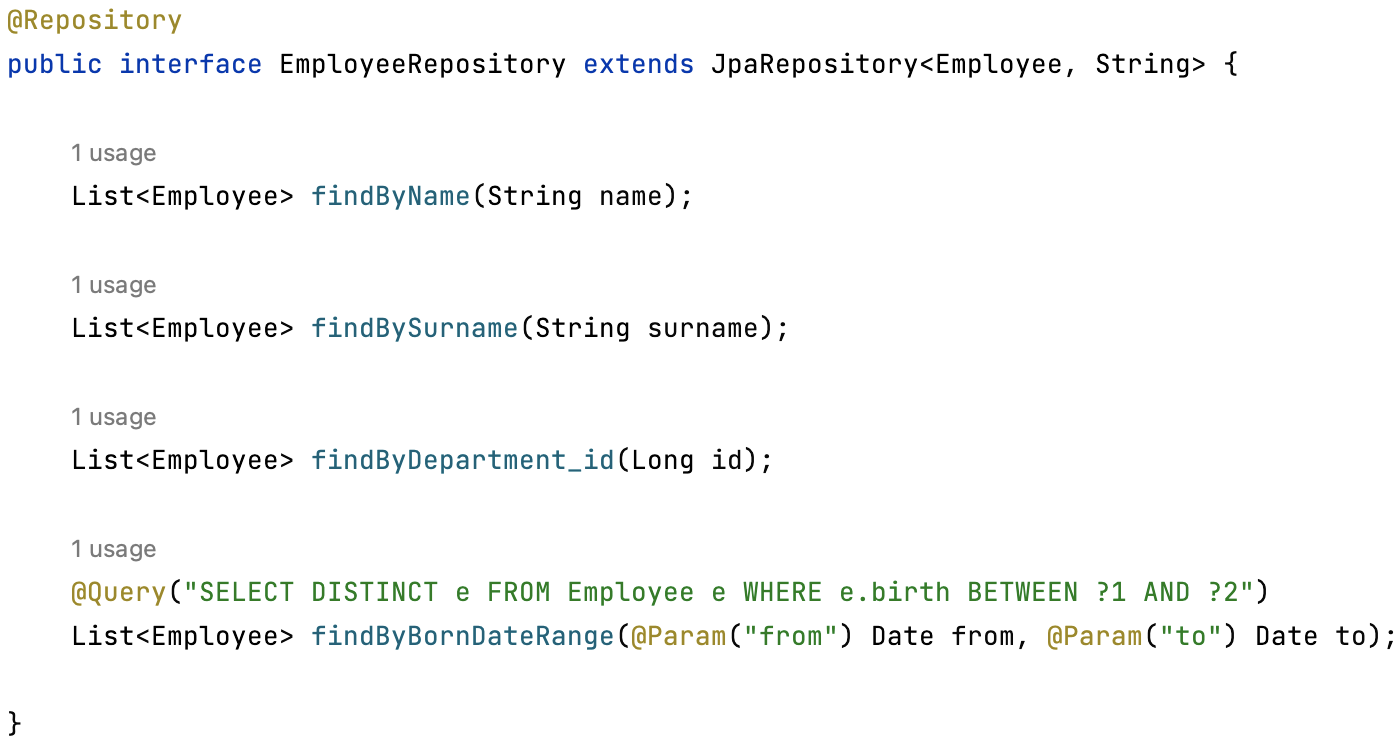
\includegraphics[width=1\linewidth]{immagini/employee_repository.png}
\caption{Esempio di implementazione della repository di Employee in Spring Boot.}
\label{employee-repository}
\end{figure}
\FloatBarrier
%%% IMG
Dunque oltre ai classici metodi di ricerca disponibili già dopo l'estensione dell'interfaccia JPARepository<T, ID>, sono stati realizzati alcuni metodi per la ricerca di impiegati per nome, per cognome e per id di dipartimento in cui lavorano. Infine è stata realizzata una query personalizzata per la ricerca di impiegati nati in un range di date.\\
Infine è possibile notare in figura \ref{employee-repository} l'annotazione \textbf{@Repository} attribuita alla'interfaccia, fondamentale al fine di indicare che la classe fornisce meccanismi per modellare i dati dell'applicativo.
\paragraph{Service}
Lo strato di servizio è lo strato che si trova tra lo strato di controller e quello di repository, il suo compito è facilitare la comunicazione tra controller e repository e inoltre contiene la business logic dell'applicativo.
Per ciascun repository, dunque per ciascuna entità, è stato realizzato un servizio specifico per gestirne le logiche.\\
Al fine di rispettare i principi SOLID della programmazione, per questioni di loose coupling e semplicità nel testing, è stato scelto di implementare il pattern secondo il quale per ogni entità viene realizzata una interfaccia del servizio ed la sua implementazione, come mostrato in figura \ref{service-serviceImpl} nel caso del servizio per l'entità Employee.
%%% IMG
\FloatBarrier
\begin{figure}[!ht]
\centering
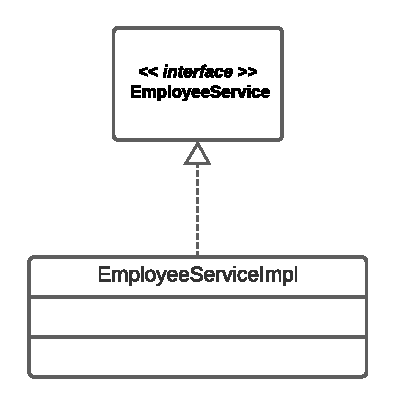
\includegraphics[width=0.3\linewidth]{immagini/service_serviceImpl.pdf}
\caption{Esempio di implementazione dell'interfaccia EmployeeService.}
\label{service-serviceImpl}
\end{figure}
\FloatBarrier
%%% IMG
Di seguito, in figura \ref{employeeServiceImpl}, viene riportato un esempio di servizio implementato, in questo caso si tratta dell'implementazione del servizio per l'Employee, ovvero della classe \textbf{EmployeeServiceImpl}.
%%% IMG
\FloatBarrier
\begin{figure}[!ht]
\begin{mdframed}
\centering
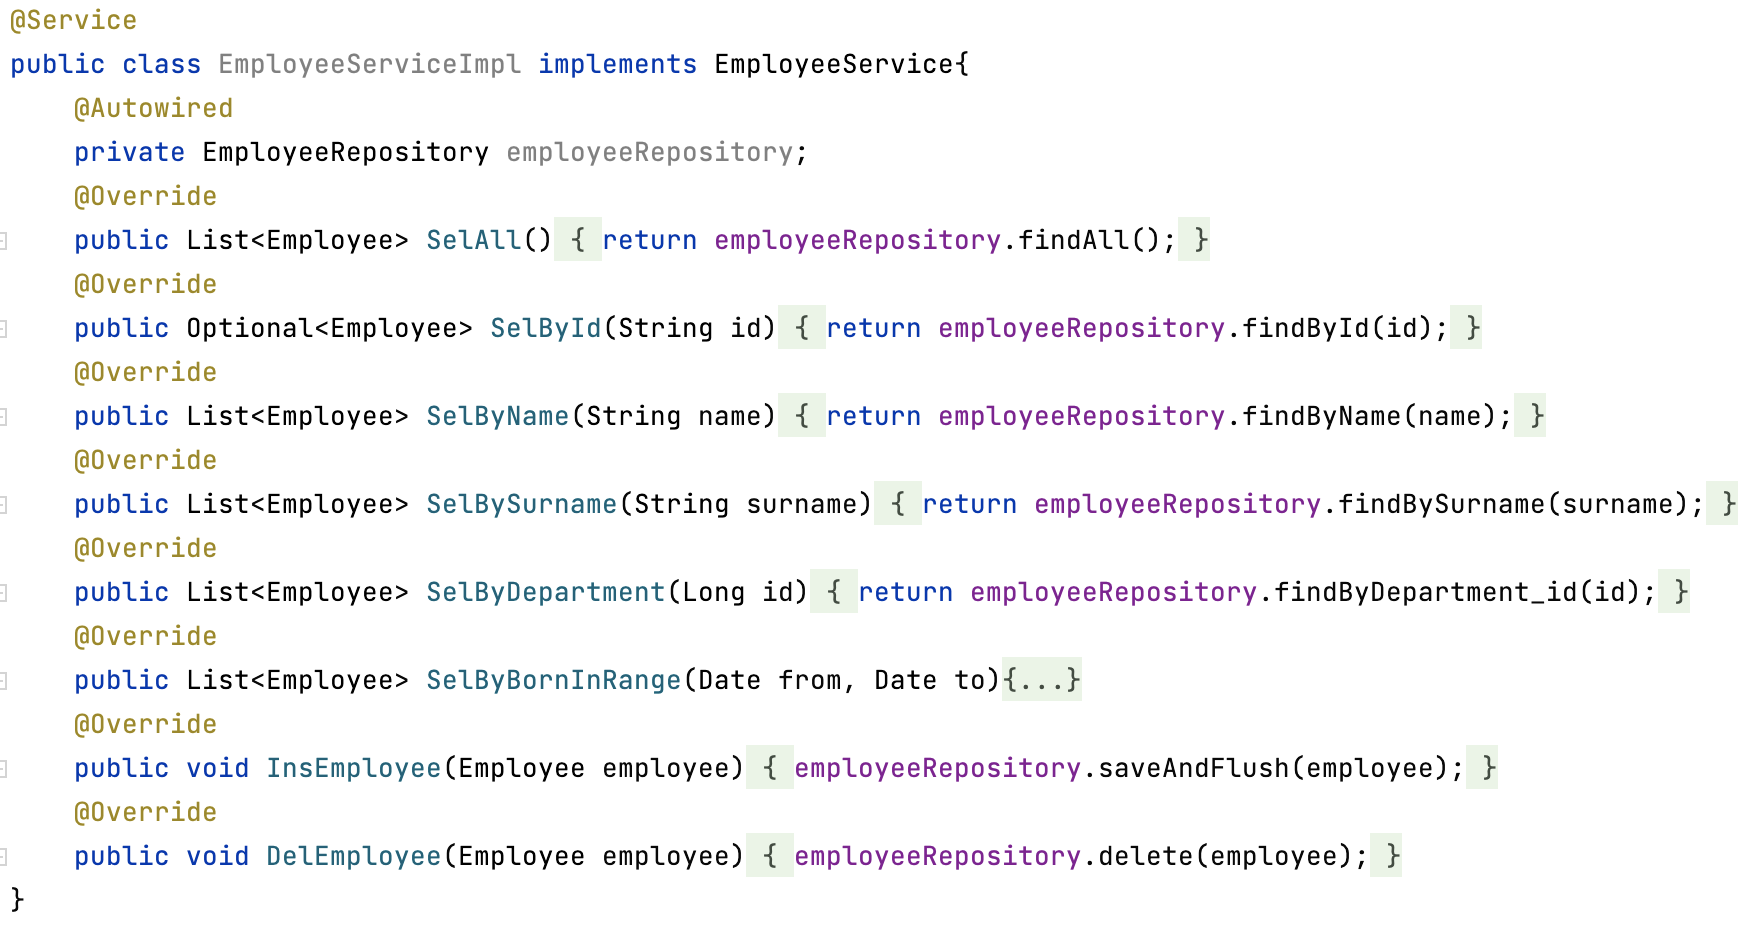
\includegraphics[width=1\linewidth]{immagini/employeeServiceImpl.png}
\end{mdframed}
\caption{Classe EmployeeServiceImpl.}
\label{employeeServiceImpl}
\end{figure}
\FloatBarrier
%%% IMG
In figura \ref{employeeServiceImpl} è possibile notare come la classe sia caratterizzata dall'annotazione \textbf{@Service} la quale viene utilizzata per indicare classi che contengono la business logic e viene utilizzata dunque per marcare la classe come service provider.\\
Continuando ed andando ad analizzare i campi dati è possibile visualizzare la dipendenza che la classe \textit{EmployeeServicImpl} ha con la repository \textit{EmployeeRepository}. In Spring questa dipendenza viene risolta con l'annotazione \textbf{@Autowired}, la quale permette di eseguire la dependency injection del bean \textit{employeeRepository}.\\
Infine sono presenti tutti i metodi, ciascuno con annotazione \textbf{@Override} poiché sono stati dichiarati anche nell'interfaccia implementata da \textit{EmployeeServiceImpl}. Sono stati resi disponibili metodi semplici che vanno ad invocare, grazie alla dipendenza con la repository, le query già disponibili con la \textit{JPARepository<T, ID>} e la query vista precedenemente \textit{SelByBornInRage}.
\paragraph{Controller}
Infine troviamo i controller, ovvero l'ultimo strato che si occupa di gestire le richieste che il server riceve attraverso il protocollo HTTP, e di mapparle inoltre ai relativi metodi. In figura \ref{employeeController} il controller di Employee, ovvero la classe \textit{EmployeeController}:
\FloatBarrier
\begin{figure}[!ht]
\begin{mdframed}
\centering
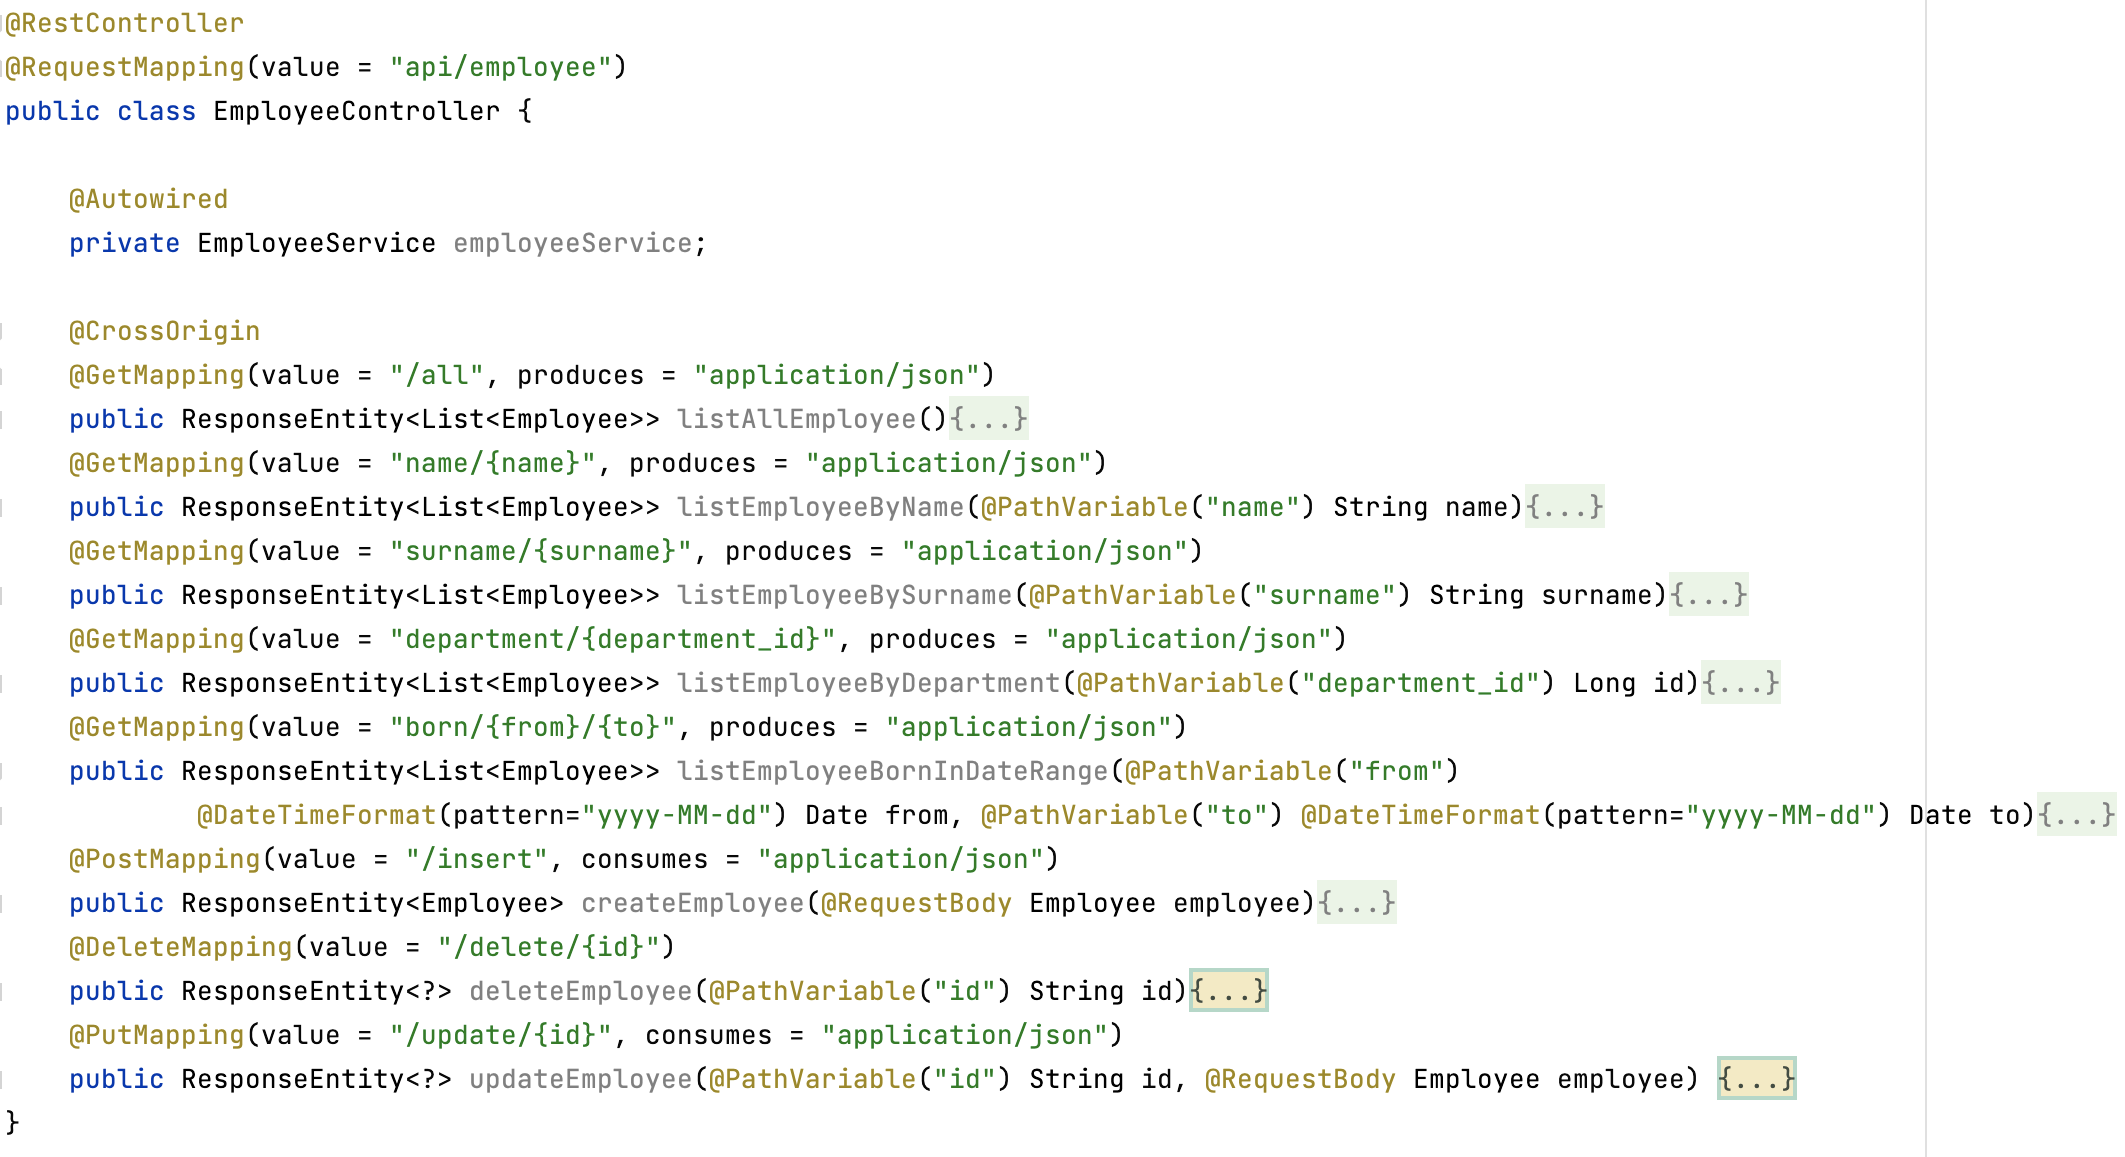
\includegraphics[width=1\linewidth]{immagini/EmployeeController.png}
\end{mdframed}
\caption{Classe EmployeeController.}
\label{employeeController}
\end{figure}
\FloatBarrier
Questa classe permette di gestire e mappare le richieste a seconda dell'url dal quale proviene la richiesta. In figura \ref{employeeController} è possibile visualizzare due annotazioni associate alla classe, l'annotazione \textbf{@RestController}, utilizzata per definire la classe come un controller di tipo REST, mentre l'annotazione \textbf{@RequestMapping} indica l'url al quale il client dovrà mandare le richieste per quello specifico controller.\\
Proseguendo è possibile indivudare una dipendenza della classe con lo strato di servizio, infatti con l'annotazione \textbf{@Autowired} e dunque con la dependency injection viene risolta la dipendenza. La classe \textit{EmployeeController} necessita una dipendenza con la classe \textit{EmployeeServiceImpl} poiché dovrà andare ad invocarne i metodi.\\
Dunque proseguendo è possibile visualizzare i vari metodi, tutti hanno una annotazione che può essere :
\begin{itemize}
  \item \textbf{@GetMapping}: indica che si tratta di un metodo per la risoluzione di una richiesta GET; specifica l'url al quale ricevere la richiesta e ciò che viene ritornato, ovvero un file JSON;
  \item \textbf{@PostMapping}: indica che si tratta di un metodo per la risoluzione di una richiesta POST, specifica l'url al quale ricevere la richiesta e ciò che richiede in input, ovvero un file JSON passato attraverso il body della richiesta HTTP;
  \item  \textbf{@DeleteMapping}: indica che si tratta di un metodo per la risoluzione di una richiesta DELETE, specifica l'url al quale ricevere la richiesta;
  \item \textbf{@PutMapping}: indica che si tratta di un metodo per la risoluzione di una richieste PUT, specifica l'url al quale ricevere la richiesta e ciò che richiede in input, ovvero un file JSON passato attraverso il body della richiesta HTTP;
\end{itemize}
Oltre alle annotazioni sopra riportate, sono presenti tra gli argomenti le annotazione \textbf{@PathVariable} la quale vuole indicare che si tratta di una variabile che verrà fornita nell'url nel posto definito dal nome specificato, \textbf{@RequestBody} ovvero un argomento che verrà fornito nel body della chiamata HTTP e infine \textbf{@DateTimeFormat} per specificare il formato del tipo di dato \textit{Date} che verrà passato dal client nell'url della richiesta.
Sono state rese dunque disponibili le seguenti query:
\begin{itemize}
  \item \textbf{listAllEmployee}: ritorna tutti gli impiegati presenti;
  \item \textbf{listEmployeeByName}: ritorna tutti gli impiegati con una determinato nome;
  \item \textbf{listEmployeeBySurname}: ritorna tutti gli impiegati con un determinato cognome;
  \item \textbf{listEmployeeByDepartment}: ritorna tutti gli impiegati di un dipartimento;
  \item \textbf{listEmployeeByBornInDataRange}: ritorna tutti gli impiegati nati in un determinato range di date;
  \item \textbf{updateEmployee}: vengono aggiornati i campi dati di un impiegato;
  \item \textbf{createEmployee}: aggiunta di un nuovo impiegato;
  \item \textbf{deleteEmployee}: rimozione di un impiegato.
\end{itemize}
\textcolor{red}{Parlare della gestione delle eccezioni con @ExceptionHandler, se ho tempo.}
\paragraph{Testing API}
Essendo un prototipo incentrato sulla realizzazione delle API, sono stati svolti in maniera semplice e veloce i test per gli strati di servizio e repository, dunque non verranno riportati. Per quanto riguarda i testi sui controller stati svolti dei test più approfonditi.\\
Per eseguire i test sui metodi del controller è stato scelto di utilizzare il framework JUnit5 \textcolor{red}{(REINDIRIZZARE AL CAPITOLO TECNOLOGIE)}.\\
Il primo test realizzato è uno \textit{SmokeTest} e da qui il nome della classe realizzata per testare che il contesto Spring abbia effettivamente creato i controller dell'applicazione. In figura \ref{smoke-test} la classe \textit{SmokeTest} con una dipendenza per ciascun controller risolta con la dependency injection grazie all'annotazione \textbf{@Autowired}. Sono poi presenti quattro metodi, uno per controller, per verificarne se sono stati creati nel contesto. Infine ciascun metodo deve essere annotato con \textbf{@Test} per indicare al framework JUnit5 che si tratta di un metodo di test.\\
Come possiamo notare sempre nell'immagine \ref{smoke-test} è presente l'annotazione \textbf{@SpringBootTest}, necessaria per indicare a Spring Boot dove si trova la principale classe di configurazione, e dunque avviare il contesto Spring. Da notare inoltre che ciascun metodo è dichiarato in maniera da poter sollevare eccezzioni se necessario.
\FloatBarrier
\begin{figure}[!ht]
\begin{mdframed}
\centering
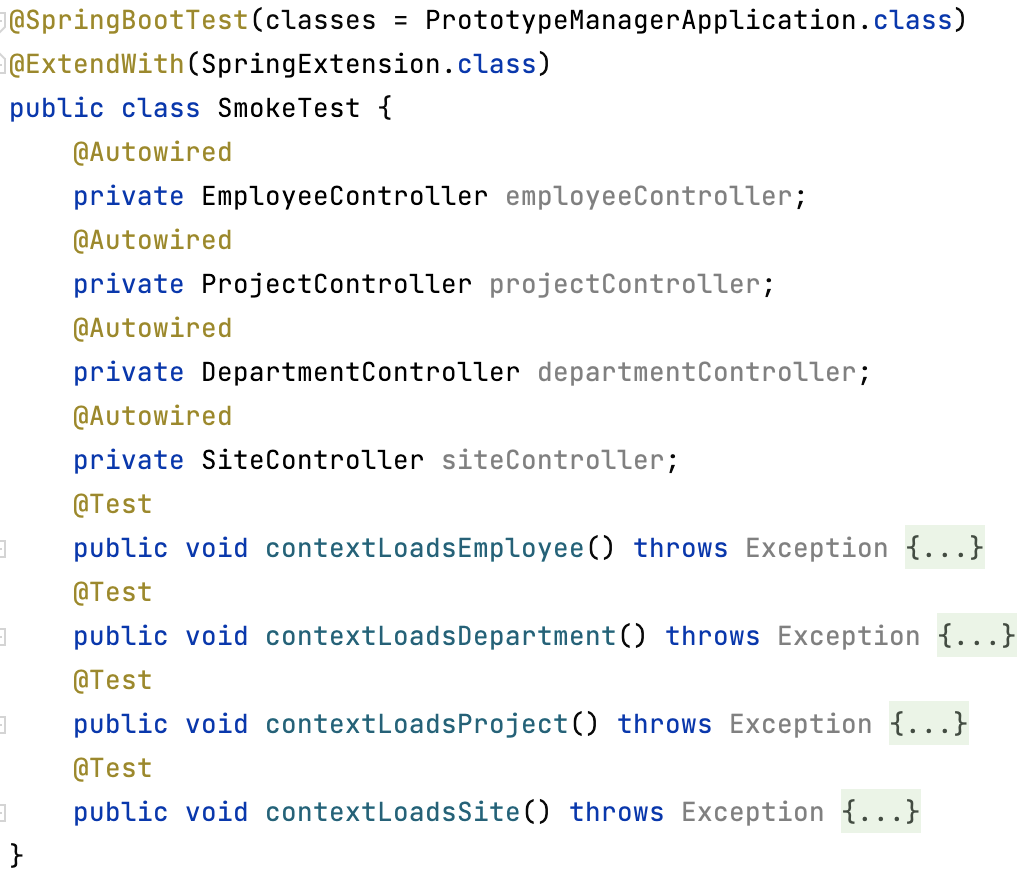
\includegraphics[width=0.7\linewidth]{immagini/SmokeTest.png}
\end{mdframed}
\caption{Classe \textit{SmokeTest} sulla creazione dei controller.}
\label{smoke-test}
\end{figure}
\FloatBarrier
Passiamo ora ai test metodi del controller \textit{EmployeeController}. Nell'immagine \ref{employee-controller-test} è raffigurata la classe \textit{EmployeeControllerTest} con metodi i vari test da effettuare sul controller.
\FloatBarrier
\begin{figure}[!ht]
\begin{mdframed}
\centering
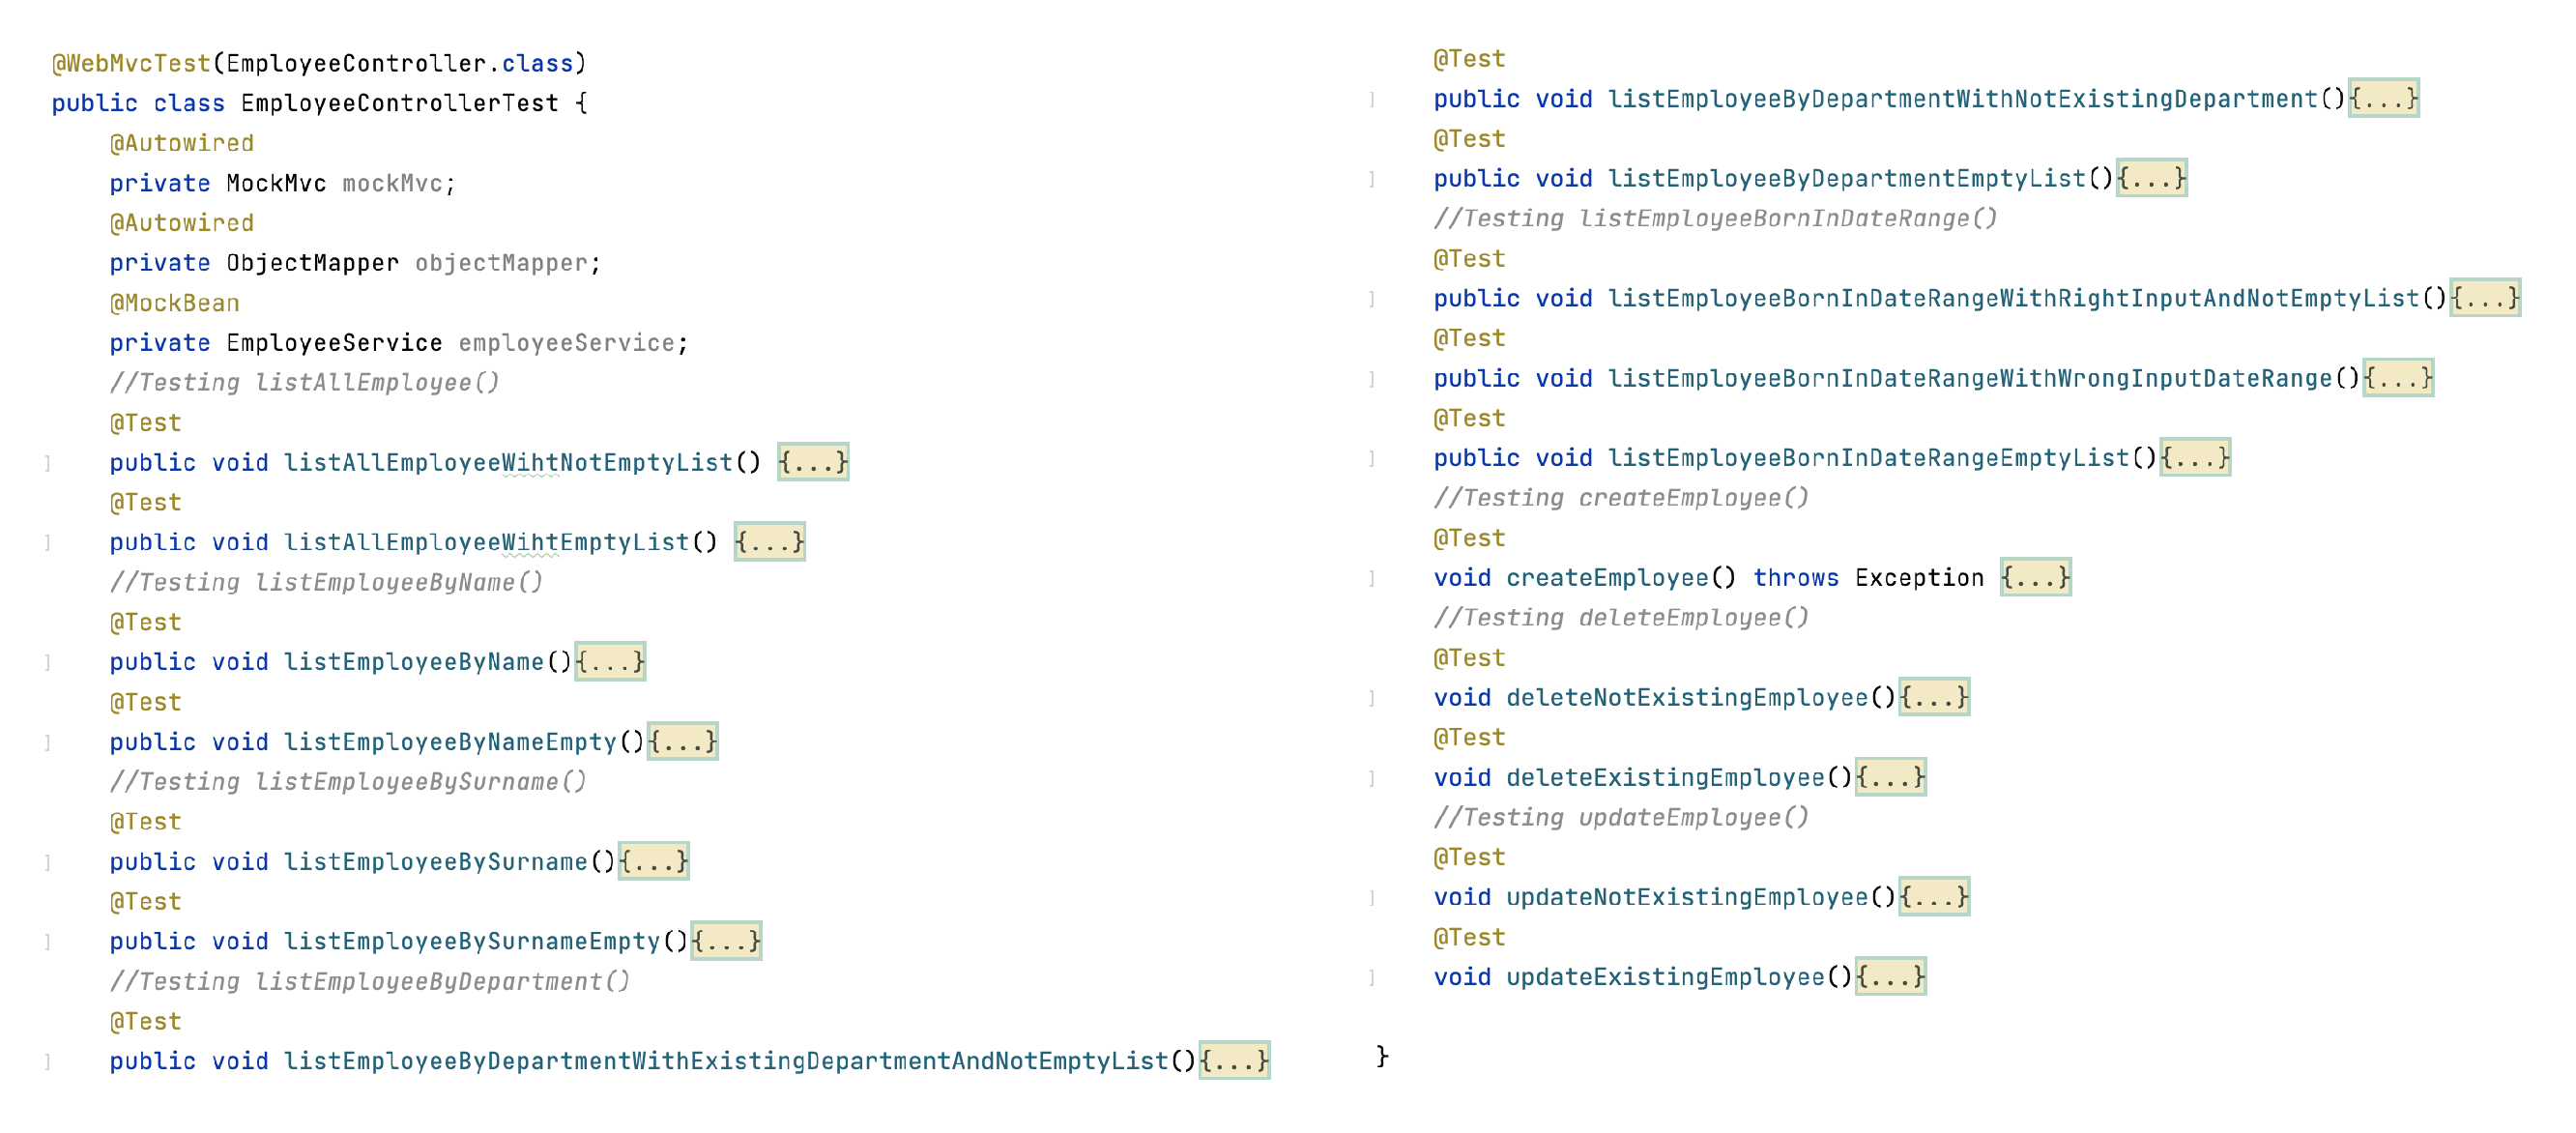
\includegraphics[width=1\linewidth]{immagini/EmployeeControllerTest.pdf}
\end{mdframed}
\caption{Classe \textit{EmployeeControllerTest}.}
\label{employee-controller-test}
\end{figure}
\FloatBarrier
Nell'immagine \ref{employee-controller-test} la classe \textit{EmployeeControllerTest} ha due annotazioni: la prima è \textbf{@WebMvcTest}, utile poiché permette di caricare nel contesto di test esclusivamente il controller di Employee e inoltre permette di tralsciare tutte le configurazioni classiche per lasciar spazio alle configurazioni di test, mentre \textbf{@ExtendWhit} permette di integrare nel contesto di test la \textit{SpringExtension} utile poiché fornisce supporto per il testing \textcolor{red}{(Non necessaria qui forse...)}.\\
Nella classe di test \textit{EmployeeControllerTest} sono dichiarate tre dipendenze fondamentali:
\begin{itemize}
  \item \textbf{MockMvc}: dipendenza risolta cona la dependency injection, viene utilizzata sucessivamente per simulare chiamate HTTP e verificarne la risposta;
  \item \textbf{ObjectMapper}: dipendenza risolta con la dependency injection, oggetto utilizzato nei test per la serializzazione e deserializzazione degli oggetti JSON in oggetti java e viceversa;
  \item \textbf{EmployeeService}: servizio che viene utilizzato nei test, per questo motivo ha l'annotazione \textbf{@MockBean}, la quale permette di aggiungere un mock dell'oggetto \textit{EmployeeService}.
\end{itemize}
Per finire la sezione sulle REST API viene di seguito riportato in figura \ref{create-employee} l'implementazione nel dettaglio del metodo di test \textit{createEmployee} seguendo il pattern \textit{Arrange - Act - Assert}.
\FloatBarrier
\begin{figure}[!ht]
\begin{mdframed}
\centering
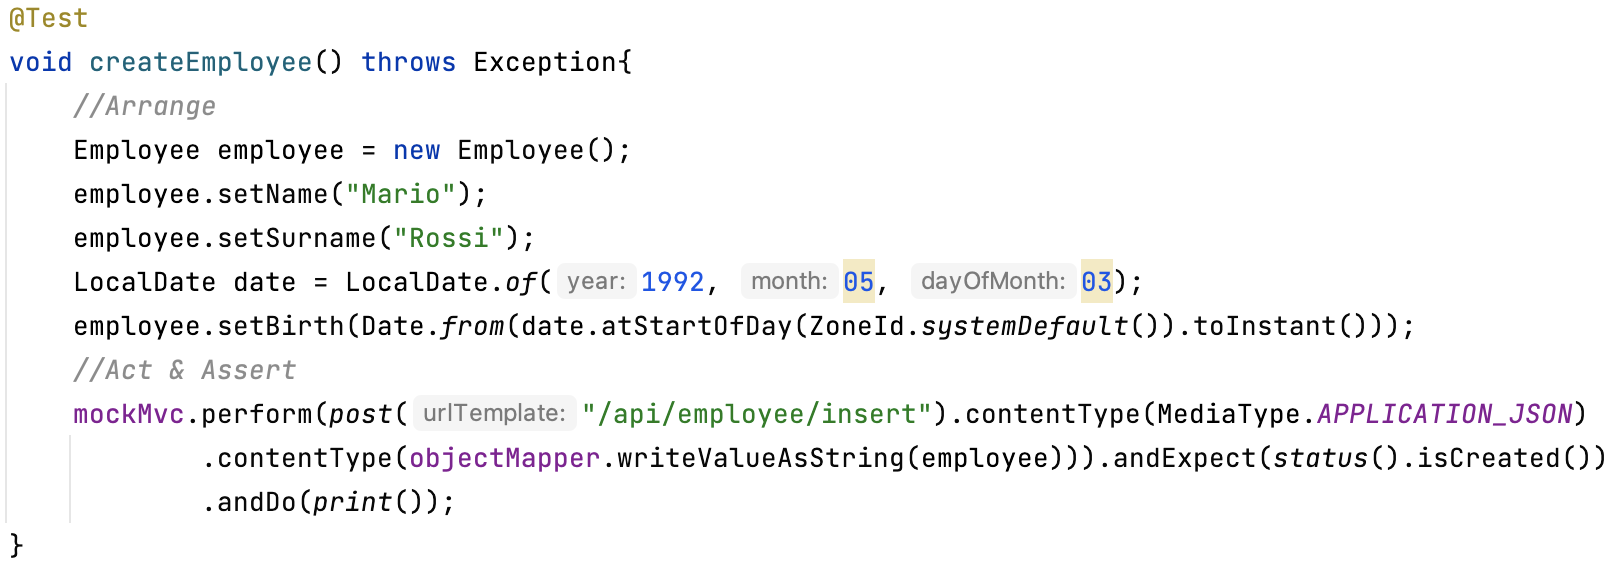
\includegraphics[width=1\linewidth]{immagini/createEmployee.png}
\end{mdframed}
\caption{Metodo di test \textit{createEmployee} della classe \textit{EmployeeControllerTest}.}
\label{create-employee}
\end{figure}
\FloatBarrier
Nella prima parte (arrange) viene creato un nuovo Employee e gli viene assegnato un nome, un cognome e una data di nascita, successivamente nella fase successiva (act), viene eseguita la chiamata GET utilizzando l'oggetto \textit{MockMvc} e passando nel body della richiesta HTTP l'oggetto Java Employee trasformato in JSON grazie all'\textit{ObjectMapper}. Infine nella fase finale (Assert), si verifica che lo stato di ritorno sia \textit{created}, in caso contrario il test fallisce.
\subsubsection*{Frontend}
Per quanto riguarda il frontend dell'applicativo è stato utilizzato il framework Angular per realizzare una single-page application. Si tratta di un frontend minimale, realizzato con il solo scopo di comprendere e sviluppare la parte di comunicazione con il server utilizzando al massimo le REST API disponibili. Per questo motivo non è stata effettuata alcuna analisi sull' utenza e sono stati tralascati completamente aspetti quali estetica grafica, accessibilità e responsive design.\\
\paragraph{Architettura}
L'architettura della web application realizzata in Angular prevede l'utilizzo del pattern Model-View-Controller:
\FloatBarrier
\begin{figure}[!ht]
\centering
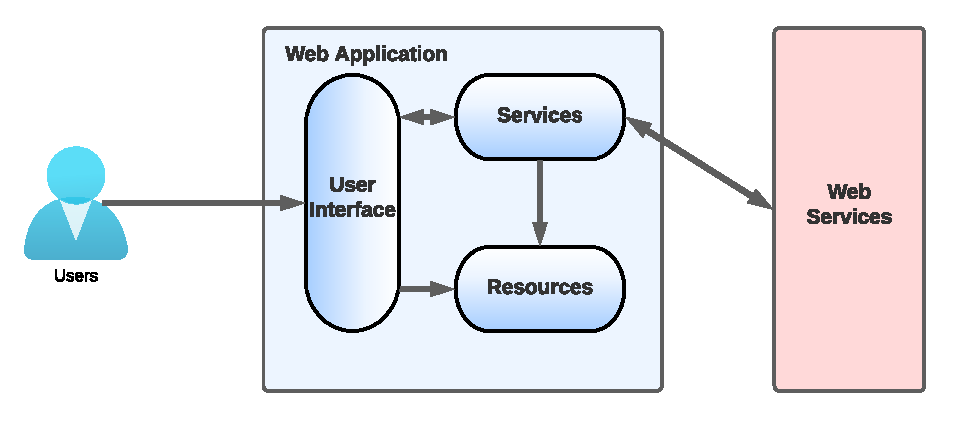
\includegraphics[width=1\linewidth]{immagini/angular_architecture.pdf}
\caption{Architettura della Web Application del prototipo.}
\label{angular-architecture}
\end{figure}
\FloatBarrier
Come visibile in figura \ref{angular-architecture} l'utente interagisce con la user interface (View) e ne modifica lo stato. Le resources (Model) vengono modificate dai services (Controller) anche su invocazione dei servizi da parte della user interface. I services sono coloro che si occupano della comunicazione con il server di backend attraverso le richiesta e risposte HTTP.
\paragraph{Funzionalità}
Per le ragioni spiegate precedentemente saranno rese disponibili nell'interfaccia grafica quelle funzionalita che andranno a permettere il massimo utilizzo delle richieste API al backend.\\
Come fatto in precedenza, verrà mostrata e spiegata esclusivamente la parte riguardante l'entità Employee per questioni di praticità, questo perché le altre entità sono state trattate in maniera analoga.\\
Dunque, in linea con le query rese disponibili dal backend riportate sulla sezione riguardante i controller, devono essere presenti le seguenti funzionalità:
\begin{itemize}
  \item \textbf{Visualizzazione degli Employee}: devono poter essere visualizzati gli impiegati in lista, o ricercati attraverso i campi: nome, cognome, data di nascita o dipartimento di appartenenza;
  \item \textbf{Aggiunta di un Employee}: deve essere possibile aggiungere un nuovo impiegato potendone specificare: nome, cognome, salario, data di nascita, dipartimento di appartenenza e infine i progetti che segue;
  \item \textbf{Aggiornamento di un Employee}: deve essere possibile aggiornare i campi dati di un impiegato specificandone l'id e il/gli campo/i da modificare;
  \item \textbf{Eliminazione di un Employee}: deve essere possibile eliminare un impiegato specificandone l'id.
\end{itemize}
Nel paragrafo sucessivo verrà mostrato come sono state implementate le funzionalità appena introdotte.
\paragraph{Implementazione FE}
Inizialmente sono state create le interfacce per poter creare gli oggetti corrispondenti alle quattro entità del prototipo. Di seguito in figura \ref{employee-interface} l'esempio della dichiarazione della interfaccia dell'entità Employee:
\FloatBarrier
\begin{figure}[!ht]
\centering
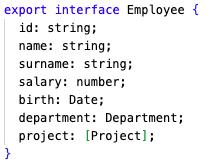
\includegraphics[width=0.3\linewidth]{immagini/employeeInterface.png}
\caption{Interfaccia di Employee.}
\label{employee-interface}
\end{figure}
\FloatBarrier
Analogamente sono state create le interfacce delle altre entità.\\
Proseguendo, è stata realizzata la realizzazione dell'interaccia grafica inserendo nella pagina iniziale la possibilità di effettuare due scelte: la prima scelta riguarda l'entità, mentre la seconda riguarda l'operazione che si vuole eseguire sull'entità selezionata. In figura \ref{first-page} è possibile visualizzare la prima pagina:
\FloatBarrier
\begin{figure}[!ht]
\centering
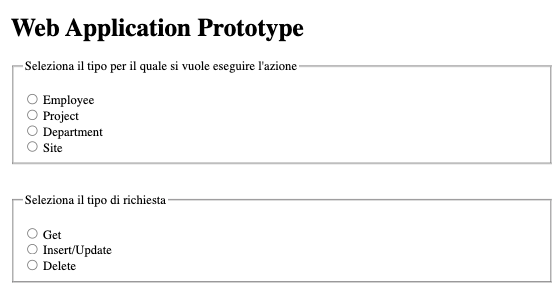
\includegraphics[width=0.7\linewidth]{immagini/firstPage.png}
\caption{Prima pagina della Web Application.}
\label{first-page}
\end{figure}
\FloatBarrier
Una volta selezionate le due opzioni viene aggiunta dinamicamente la possibilità di specificare i dettagli della richiesta. Considerando solo l'entità Employee per le ragioni spiegate precedentemente, vengono di seguito mostrate le diverse interfacce che variano al variare della scelta selezionata e il servizio che permette di eseguire la chiamata alle API del backend.\\
In figura \ref{get-employee}abbiamo il caso in cui è stato selezionata l'entità Employee con operazione GET:
\FloatBarrier
\begin{figure}[!ht]
\centering
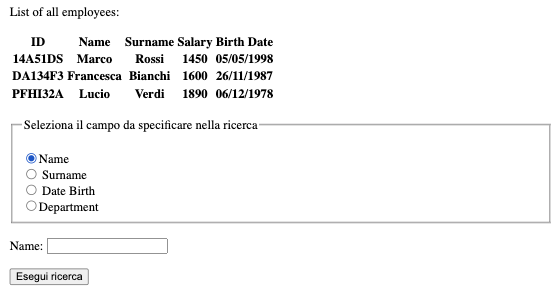
\includegraphics[width=0.7\linewidth]{immagini/getEmployee.png}
\caption{Opzioni disponibili con operazione GET selezionata.}
\label{get-employee}
\end{figure}
\FloatBarrier
Viene dunque visualizzata immediatamente una lista contenente tutti gli impiegati, per ciascun impiegato vengono mostrati id, nome e cognome, salario e data di nascita. Successivamnete viene visualizzata la scelta riguardante il campo per il quale eseguire la ricerca, in questo caso è stato scelto il nome, dunque inserendo nell'apposito campo di input il nome e selezionendo il bottone è possibile effettuare la ricerca per nome.\\
La scelta dell'opzione get permette alla vista di invocare immediatamente il servizio che esegue una chiamata alle REST API del backend per ricevere la lista di tutti gli employee, stessa cosa accade anche quando premiamo il bottone "Esegui ricerca " dopo aver inserito il nome. Il servizio in questione si chiama \textit{EmployeeService} e di seguito in figura \ref{employee-service} ne è riportata l'implementazione:
\FloatBarrier
\begin{figure}[!ht]
\centering
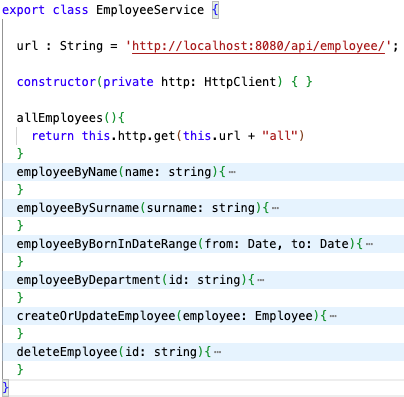
\includegraphics[width=0.6\linewidth]{immagini/employeeService.png}
\caption{Classe \textit{EmployeeService}.}
\label{employee-service}
\end{figure}
\FloatBarrier
Il servizio realizzato per le chiamate alle REST API del backend, permette di essere invocato direttamente dalla vista alla selezione di un elemento HTML.\\\\
Proseguendo vengono visualizzati ora i casi in cui si sceglie come operazione quella di modificare o aggiungere un nuovo impiegato. In figura \ref{post-employee} è possibile visualizzare la porzione di interfaccia grafica per l'inserimento o l'aggiornamento di un impiegato:
\FloatBarrier
\begin{figure}[!ht]
\centering
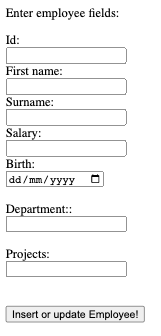
\includegraphics[width=0.3\linewidth]{immagini/postEmployee.png}
\caption{Opzioni disponibili con operazione Insert/Update selezionata.}
\label{post-employee}
\end{figure}
\FloatBarrier
Dunque una volta inseriti tutti i valori per ciascun campo, tranne il campo ID che viene generato automaticamente, è possibile aggiungere un nuovo impiegato. Qualora invece si specificasse anche l'id, allora si tratterebbe di una modifica di un employee già esistente, questo solo se l'id inserito corrisponde veramente all'id di un employee. Anche in questo caso selezionando il bottone "Insert or update Employee!" viene invocato il metodo del servizio riportato in figura \ref{employee-service}.\\
Per finire in figura \ref{delete-employee} il caso in cui venga selezionata l'opzione delete:
\FloatBarrier
\begin{figure}[!ht]
\centering
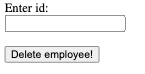
\includegraphics[width=0.3\linewidth]{immagini/deleteEmployee.png}
\caption{Opzioni disponibili con operazione Delete selezionata.}
\label{delete-employee}
\end{figure}
\FloatBarrier
\paragraph{Testing FE}
I test di unità sono stati implementati seguendo il pattern \textit{Arrange - Act - Assert} sui metodi del servizio riportato in figura \ref{employee-service}. Di seguito nell'immagine \ref{employee-service-tests} è possibile visualizzare la funzione \textit{describe} la quale viene utilizzata per raggruppare un insieme di test:
\FloatBarrier
\begin{figure}[!ht]
\centering
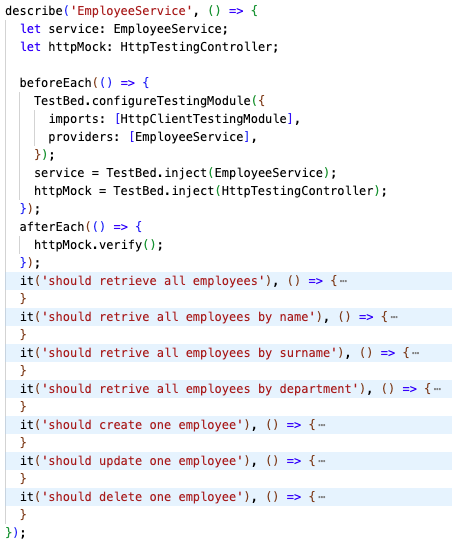
\includegraphics[width=0.6\linewidth]{immagini/employeeServiceTest.png}
\caption{Test per i metodi del servizio \textit{EmployeeService}.}
\label{employee-service-tests}
\end{figure}
\FloatBarrier
Viene utilizzato il modulo Angular \textit{HttpClientTestModule}, necessario al fine di importare il servizio inettabile \textit{HttpTestingController}, utilizzato per il mocking e il flushing per eliminare le microtasks in sospeso. Sono inoltre presenti le funzioni \textit{BeforeEach()} utilizzata per configurare l'ambiente di test, dunque importare i moduli necessari e risolvere le dipendenze, e la funzione \textit{afterEach()} utilizzata per controllare, dopo l'esecuzion di ciascun test, che non siano rimaste richieste in sospeso. Infine, con la funzione \textit{it()} viene definito un titolo per ciascun test e viene implementato il test.\\
Più nello specifico in figura \ref{get-all-test} si può visualizzare l'implementazione di un test per il metodo \textit{allEmployee} del servizio \textit{EmployeeService}:
\FloatBarrier
\begin{figure}[!ht]
\centering
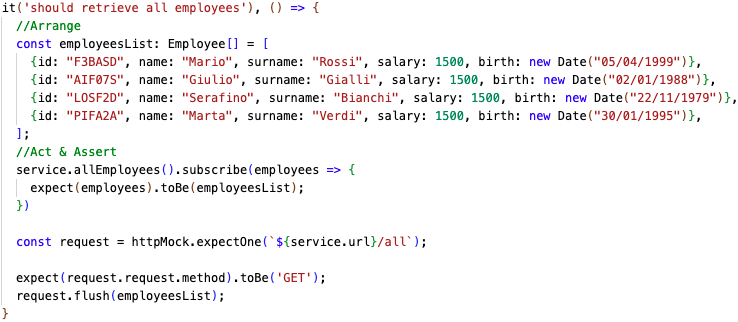
\includegraphics[width=0.8\linewidth]{immagini/allEmployeeTest.png}
\caption{Test sul metodo \textit{allEmployee()} di \textit{EmployeeService}.}
\label{get-all-test}
\end{figure}
\FloatBarrier
Viene inizialmente creato un array di Employee che ci si aspetterà di ricevere dalla chiamata, e sucessivamente viene controllato un test per verificare che ciò accada effettivamente con la funzione \textit{expect()}. Infine viene controllato che l'url sia corretto, che venga effettuata una sola chiamata GET e che si tratti effettivamente di una richiesta GET.

\subsection{Migrazione da REST a GraphQL}
Nella seguente sottosezione verrà mostrato come è stato migrato sia il backend che il frontend del prototipo realizzato da REST API a GraphQL API.
\subsubsection*{Migrazione Backend}
Il backend realizzato in Spring Boot con l'aiuto del modulo Spring Data REST per la realizzazione dei controller di REST API, deve essere riscritto in parte utilizzando il modulo Spring GraphQL per la realizzazione dei controller in GraphQL.\\
Seguendo la metodologia \textit{Schema First} la prima cosa che è stata creata è il GraphQL Schema.
\paragraph{GraphQL Schema}
Il GraphQL Schema è necessario al fine di definire i tipi, le query, le mutation e le subscription che il server GraphQL renderà disponibili al client.\\
Inizialmente è necessario fare un'analisi sulle enetità presenti e comprendere quali entità riportare nel GraphQL Schema. Infatti non tutte le entità devono essere necessariamente riportate nel GraphQL Schema, ma andranno riportate solo le entità che verranno utilizzate API. Nel caso del prototipo le quattro entità presenti, ovvero Employee, Project, Department e Site devono essere riportate tutte nel GraphQL schema poiché sono tutte accessibili dal client.\\
Partendo dunque dalle quattro entità, sarà necessario riportarle nel GraphQL Schema, sia come entità di input che di output nelle query, questo è necessario poiché GraphQL distingue i due tipi. In figura \ref{employee-schema} è possibile visualizzare l'implementazione dell'entità \textit{Employee} e \textit{EmployeeInput}.
\FloatBarrier
\begin{figure}[!ht]
\centering
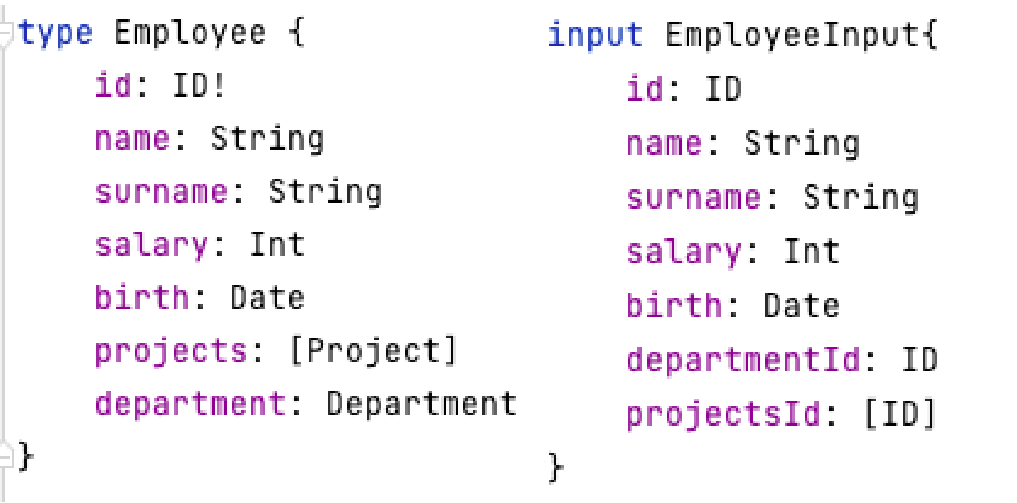
\includegraphics[width=0.8\linewidth]{immagini/employeeSchema.pdf}
\caption{Tipi \textit{Employee} e \textit{EmployeeInput} nel GraphQL Schema.}
\label{employee-schema}
\end{figure}
\FloatBarrier
Come si può notare i due tipi \textit{Employee} e \textit{EmployeeInput} non corrispondono completamente. Infatti i campi \textit{projects} e \textit{department} di \textit{Employee} non sono presenti in \textit{EmployeeInput}, o  meglio sono presenti ma in diversa forma. Questo è dovuto al fatto che il tipo \textit{Employee} è un tipo che verrà ritornato al client su richiesta, dunque dovrà contenere le varie istanze dei progetti a cui un impiegato sta partecipando e anche l'oggetto dipartimento. Mentre per quanto riguarda il tipo \textit{EmployeeInput} che corrisponde al tipo di input per l'impiegato, qualora ad esempio il client volesse creare attraverso una mutation un nuovo impiegato, sarà sufficiente specificare l'id del dipartimento in cui lavora o gli id dei progetti ai quali sta partecipando, non serve passare l'interno oggetto Project o Department.\\
Prima di passare alla dichiarazione di query, mutation e subscription, è necessario prima parlare dei tipi unione, utilizzati per gestire gli errori e poter ritornare al client un errore personalizzato ed evitare dunque che vengano ritornati gli errori incomprensibili dal GraphQL Server. Per far ciò è stato creato una interfaccia \textit{Message} e cinque tipi che la implementano e rappresentano i possibili errori o il caso di successo dell'operazione richiesta dal client, vedi figura \ref{message-interface}.
\FloatBarrier
\begin{figure}[!ht]
\centering
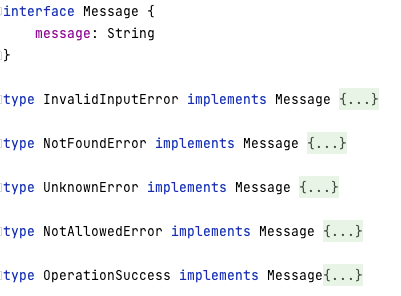
\includegraphics[width=0.6\linewidth]{immagini/messageInterface.png}
\caption{Interfaccia \textit{Message} e definizione dei tipi che la implementano nel GraphQL Schema.}
\label{message-interface}
\end{figure}
\FloatBarrier
A questo punto vengono dichiarati i tipi di unione necesssari nella realizzazione delle query e mutation che verranno dichiarate in seguito. In figura \ref{union-types} è possibile visualizzare l'implementazione dei tipi unione.
\FloatBarrier
\begin{figure}[!ht]
\centering
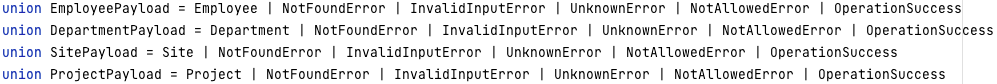
\includegraphics[width=1\linewidth]{immagini/unionType.png}
\caption{Interfaccia \textit{Message} e definizione dei tipi che la implementano nel GraphQL Schema.}
\label{union-types}
\end{figure}
\FloatBarrier
A questo punto è possibile definire le query, le mutation ed eventualmente le subscription che si vogliono rendere disponibili al client. In figura \ref{query-employee} è possibile visualizzare la dichiarazione delle query, mutation e della subscription riguardanti l'entità Employee.
\FloatBarrier
\begin{figure}[!ht]
\centering
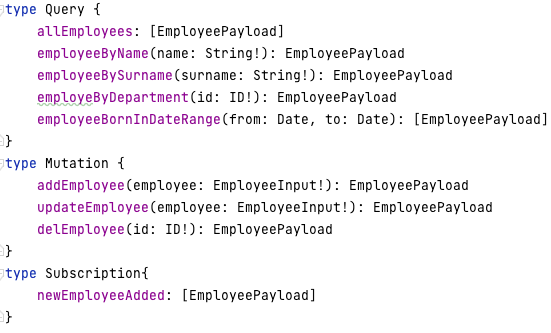
\includegraphics[width=0.6\linewidth]{immagini/queryEmployee.png}
\caption{Implementazione delle query, mutation e subscription nel GraphQL Schema.}
\label{query-employee}
\end{figure}
\FloatBarrier
Come è possibile notare sono state rese disponibili le medesime query e mutation rese disponibili nelle REST API. Il tipo di ritorno è il tipo unione \textit{EmployeePayload}, così facendo è possibile ritornare oltre che l'impiegato o gli impiegati richiesti, anche i messaggi d'errore specifici o di successo della richiesta.\\
È stata aggiunta inoltre una subscription per sfruttare a pieno le funzionalità di GraphQL. Questa subscription permette dunque, come spiegato nel capitolo \ref{protocolli-trasmissione-dati}, che il client riceva i nuovi impiegati aggiunti senza per forza richiederli.\\

\paragraph{Controller refactoring}
A questo punto resta solo la riscrittura dei controller, questo perché gli strati di servizio e repository durante la migrazione possono rimanere invariati, infatti le logiche del server e l'accesso e la gestione del database rimangono invariati. Tuttavia prima di analizzare l'implementazione del controller GraphQL, è necessario dichiarare le classi Java corrispondenti ad i vari errori ed ai tipi di input; questo è necessario poiché qualora dovessere essere ritornato un errore o dovesse essere ricevuto in input ad esempio il tipo dichiarato precedentemente \textit{EmployeeInput}, il quale non corrisponde al tipo Employee dichiarato in Java, si creerebbero degli errori durante il mapping tra i tipi Java e i tipi dichiarati nel GraphQL Schema. Per questo motivo è stato dichiarato un Java record per ciascun errore/successo, più le classi relative ai vari tipi di input.\\
L'implementazione del controller risulta differente rispetto a quella vista con le REST API. Di seguito in figura \ref{graphql-controller} è possibile visualizzarne la struttura ed i metodi:
\FloatBarrier
\begin{figure}[!ht]
\centering
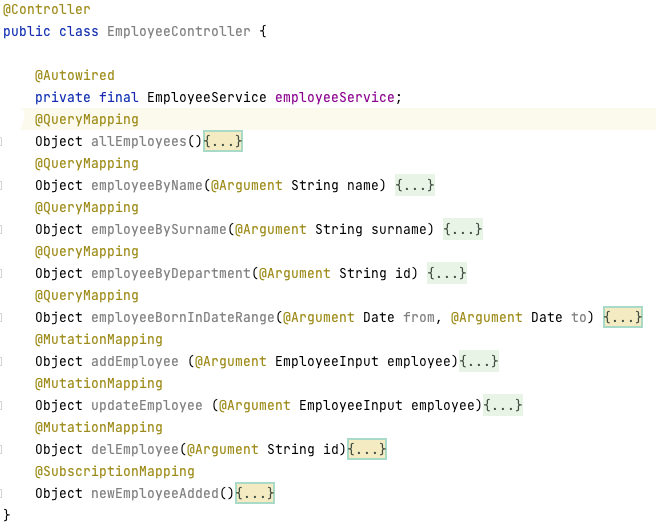
\includegraphics[width=0.8\linewidth]{immagini/graphQLEmployeeController.png}
\caption{Classe \textit{EmployeeController}.}
\label{graphql-controller}
\end{figure}
\FloatBarrier
Come si può notare in figura \ref{graphql-controller} si tratta di un controller differente rispetto al controller REST. Innanzitutto ha l'annotazione \textbf{@Controller} e non @RestController, poiché quest'ultima serve per indicare esclusivamente Spring Controller per REST API, mentre la prima è più generica ed indica esclusivamente che si tratta di un controller. Poi è possibile notare come le annotazioni sui metodi siano differenti, per le query si usa l'annotazione \textbf{@QueryMapping}, per le mutation l'annotazione \textbf{@MutationMapping}, mentre per le subscription l'annotazione \textbf{@SubscriptionMapping}, infine per gli argomenti dei metodi l'annotazione \textbf{@Argument}. Queste annotazioni sono fondamentali poiché permettono di effettuare il mapping tra i tipi, query, mutation o subscription definiti nel GraphQL Schema e quelli definiti nel controller. Per questo motivo il nome di ciascun metodo o tipo negli argomenti deve corrispondere esattamente al nome nel GraphQL Schema, altrimenti il mapping non andrà a buon fine e verranno generati degli errori.\\
In figura \ref{employee-by-name-graphql} è possibile visualizzare un esempio di implementazione di un metodo del controller, in questo caso si tratta del metodo \textit{employeeByName} il quale ritorna un errore \textit{NotFoundError} nel caso non venisse trovato alcun impiegato con il nome specificato, oppure una lista di impiegati con quel determinato nome.
\FloatBarrier
\begin{figure}[!ht]
\centering
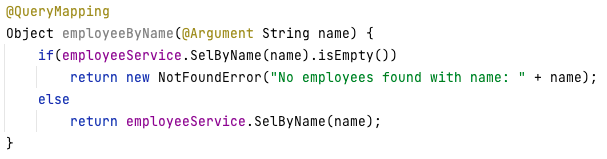
\includegraphics[width=0.8\linewidth]{immagini/employeeByNameGraphQL.png}
\caption{Metodo \textit{employeeByName} del controller \textit{EmployeeController}.}
\label{graphql-controller}
\end{figure}
\FloatBarrier
Infine, trattandosi di una particolare funzionalità disponibile esclusivamente in GraphQL, in figura \ref{subscription-graphql} è possibile visualizzare l'implementazione della subscription \textit{newEmployeeAdded}:
\FloatBarrier
\begin{figure}[!ht]
\centering
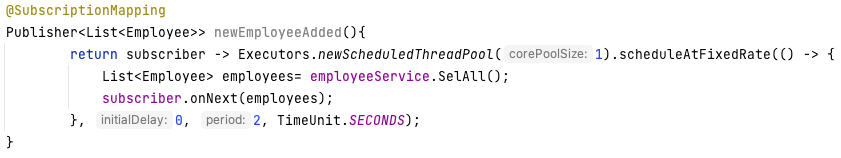
\includegraphics[width=0.8\linewidth]{immagini/newEmployeeAdded.png}
\caption{Subscription \textit{newEmployeeAdded}.}
\label{graphql-controller}
\end{figure}
\FloatBarrier
% Spiego come è stata realizzata la migrazione da REST a GraphQL. Partendo da backend, viene realizzata un'analisi sui tipi necessari da riportare nel GraphQL schema (tipi di input e tipi di ritorno). Sucessivamente vengono ristrutturate le API rese disponibili in REST (non sempre i metodi dei controller REST corrispondono a quelli GraphQL, oltre a differenze nelle annotazioni, ecc...). Vengono dunque implementati i metodi dei controller GraphQL, soffermarsi sulle difficoltà riscontrate nel mapping dei tipi GraphQL schema con i tipi corrispondenti del BE. Una volta ricostruito tutto il sistema di query GraphQL nel BE e testato, si può passare alla migrazione frontend. Volendo dividere il tutto in subsubsection:
%\begin{itemize}
%  \item analisi sui tipi;
%  \item ristrutturazione API secondo principi GraphQL;
%  \item realizzazione API con tool Spring GraphQL (e problemi mapping tipi);
%  \item testing;
%\end{itemize}
\subsubsection*{Migrazione Frontend}
%La migrazione su FE è molto più semplice rispetto al BE, infatti è sufficiente andare ad aggiornare lo strato di servizio, il quale si occupa della gestione della chiamate API al BE. Anche qui si possono riscontrare alcuni problemi per quanto riguarda la corrispondenza dei tipi (ma ho avuto più problemi in SushiLab, qui trascurabile dunque).
%Volendo dividere il tutto in subsubsection:
%\begin{itemize}
%  \item aggiornamento strato servizio con modulo apollo;
%\end{itemize}
%Questo capitoletto conterrebbe tutto, da come costruire la query a seconda di ciò che è necessario, all'eliminazione della parte di gestione delle risorse nel protitipo REST (per questioni di under e overfetching).

\section{SushiLab}
\label{sushi-lab}
\subsection{Comprensione dell'applicativo}
Breve panoramica su SushiLab, ambito d'uso, funzionalità, ecc...
\subsubsection{Panoramica del backend}
Panoramica su architettura del backend (sviluppato in Spring), entità e relazioni, business logic, strato di persistenza, test, \textbf{API} (Parte preponderante della panoramica sul backend).
\subsubsection{Panoramica del frontend}
Panoramica su architettura del frontend (sviluppato in Angular), principali components, \textbf{strato di servizio} (parte preponderante perché gestisce le chiamate alle API del backend).
\subsection{Migrazione del BE da REST a GraphQL}
Molto simile a quanto scritto per il prototipo nella parte di migrazione adattato alle API specifiche di SushiLab.
\subsection{Migrazione del FE da REST a GraphQL}


% \subsection{Progettazione }
% Tecnologie scelte per lo sviluppo del protitipo (poi espresse meglio in capitoli successivi).
% Viene spiegata l'architettura del software che si vuole realizzare (diviso per BE e FE), le entità e relative relazioni.
% \subsection{Business logic - BE}


% \subsection{Sviluppo API}
% Panoramica su quali api vengono rese disponibili da BE.
% \subsubsection{Sviluppo REST API}
% Come vengono implementate con protocollo REST.
% \subsubsection{Sviluppo GraphQL API}
% Come vengono implementate con protocollo GraphQL.
% \subsection{Comparazione dei due protocolli}
% Illustrazione delle differenze (con vantaggi e svantaggi) individuate nelle varie fasi di realizazzione del
% prototipo (analisi, progettazione, sviluppo, testing, ...). Si tratta di:
% \begin{itemize}
%         \item differenze architetturali del prototipo (dunque come sono strutturati BE e FE a seconda della tecnologia utilizzata, differenze lievi ma presenti);
%         \item differenze legate alla natura dei protocolli (ad es. che GraphQL non usa i codici di stato http classici),dunque come si rispecchiano queste differenze nel concreto (ad es. gestione differente degli errori) ;
%         \item differenze negli strumenti utilizzati (ad es. differenti librerie).
% \end{itemize}
% \section{SushiLab}
% \subsection{Comprensione della struttura e delle logiche della webapp}
% Descrizione di BE e FE della webapp, sue entità, relazioni e logica di base.
% \subsection{Migrazione BE da REST a GraphQL}
% \subsubsection{Analisi delle componenti da modificare}
% Ad esempio i metodi i controller.
% \subsubsection{Realizzazione della migrazione}
% Come ogni componente varia durante tutta la migrazione.
% \subsubsection{Difficoltà riscontrate durante la migrazione}
% Problemi riscontrati nel passaggio da REST a GraphQL (ad es. problemi legati alla forte tipizzazione di GraphQl).
% \subsection{Migrazione FE da REST a GraphQL}
% Stessa cosa del BE, probabilmente sarà molto più breve.
% \subsubsection{Analisi delle componenti da modificare}
% \subsubsection{Realizzazione della migrazione}
% \subsubsection{Difficoltà riscontrate durante la migrazione}
% \subsection{Analisi comparativa}
% Analisi comparativa della webapp nelle due versioni. Vantaggi e svantaggi della webapp due versioni sotto tutti i punti di vista:
% \begin{itemize}
%         \item complessità dei protocolli e dunque i costi per la realizzazione di una versione rispetto all'altra;
% \end{itemize}


% Volendo aggiungo anche un analisi prestazionale riportando i risultati del load testing.
% \subsection{Considerazioni finali}
% Perché in questo caso d'uso specifico ha più senso utilizzare un protocollo rispetto che l'altro.
